\section{WR Transparent Clocks}
\label{sec:wr_tc}
PTP Transparent Clock (TC) modifies PTP messages as they pass through them
adding the residence time to an accumulative Correction Field (CF) in the PTP 
messages. Thus, the delay introduced  by the network is measured and can be 
subtracted in the slave clock, which improves distribution accuracy.

In ~\ref{sec:wr} the WRPTP and WR synchronization steps has been described for
master, slave and boundary clock. In this chapter the author presents how a
standard TC becomes a WR TC.

\begin{figure*}[!t]
\centering
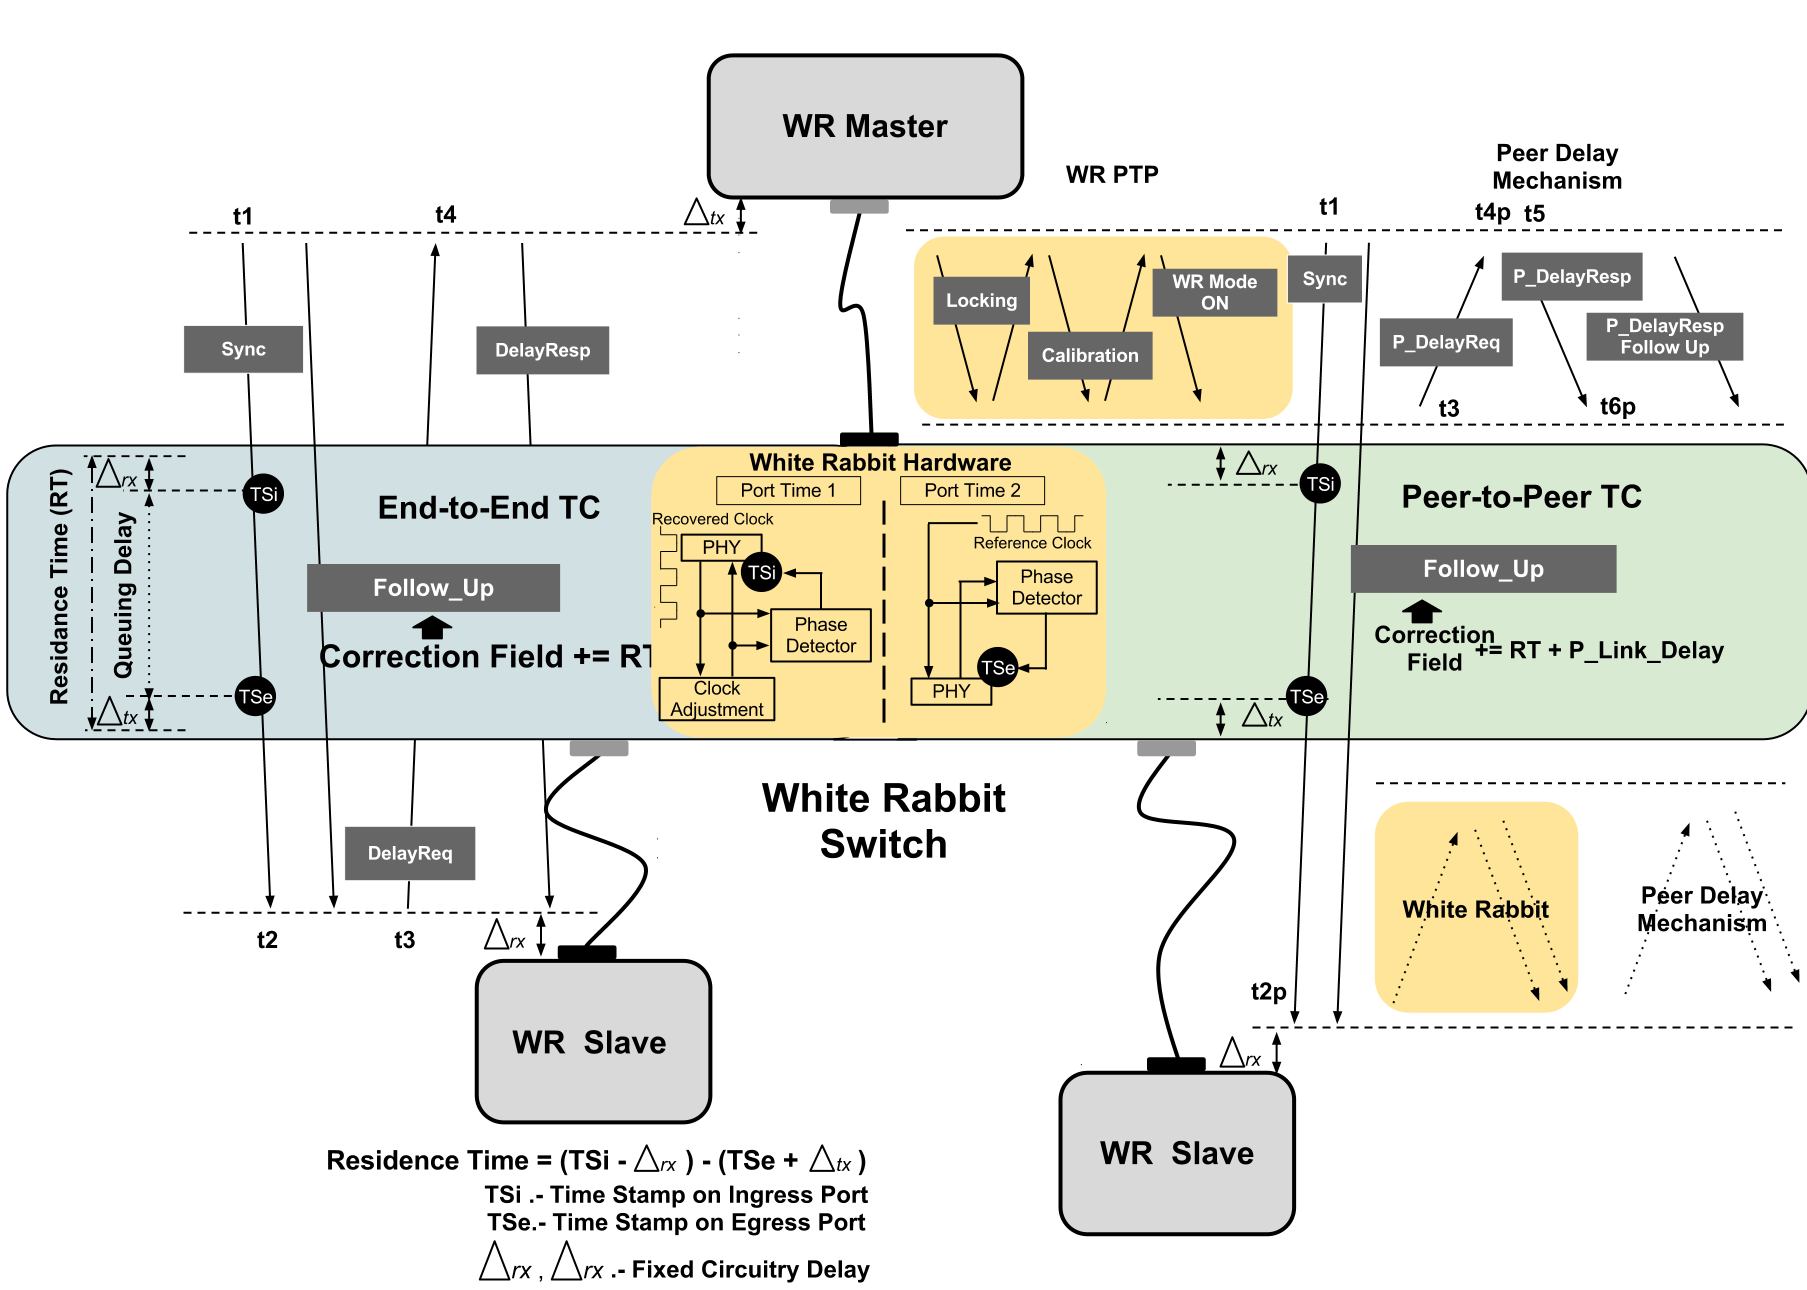
\includegraphics[scale=0.27]{fig/wr_schema_hw_bw.png}
\caption{WR E2E and P2P Transparent Clocks}
\label{fig:wr_tc}
\end{figure*}

\subsection{End-to-End WR Transparent Clock}

As the standard End-to-End (E2E) clocks, the WR E2E TC doesn't belong to the
master-slave hierarchy and does not synchronized to the WR Master. 
Therefore, a WR E2E accomplishes only the synthonization and the calibration,
the WR Mode is on, but there is no enhancement of the time stamps since the  
$delay_{ms}$ is calculated end to end, between master and slave, and there is 
not $phame_{mm}$ or $phase_{s}$ measurement. 

Thanks to the synthonization done during the WRPTP there is not errors in the 
measurement of the residence time and in the CF. 

The figure ~\ref{fig:wr_tc} shows the PTP exchange of messages from master to slave,
going transparently and how the residence time is also calculated taking into 
account the fixed delays $\Delta$. A two-step WR E2E TC calculates, using
(\ref{eq:delayms}), the $offset_{ms}$:

\begin{equation}
    \label{eq:wre2e}
     CF += (TS_{ingess\_port} - \Delta_{rx}) -
     (TS_{egress\_port} + \Delta_{tx})
\end{equation}

\begin{equation}
    \label{eq:wre2e}
     offset_{ms} = t_{1} - t_{2} - delay_{ms} - CF
\end{equation}

\subsection{Peer-to-Peer WR Transparent Clock}

As the standard Peer-to-Peer (P2P) clocks, the WR P2P TC measures residence time
of Sync messages, and the link delay in both directions. Since the link delay
is done between adjacent clocks using the peer delay mechanism, the fully WR synchronization
process can be issued between the two ports. The figure ~\ref{fig:wr_tc} shows how the
WR P2P initiates on after sides of the TC.

The measurement of the residence time, like in the E2E should suffer no error
since the ports are syntonized to its master clock, but also the measurement of the
link delays, are as precise as the WR project claims ~\cite{biblio:ispcs_m} for the
Boundary Clocks. The link delay is calculate like in (\ref{eq:delayms}) and the
fig ~\ref{fig:time_stamp} shows, but using $t_{3}$, $t_{4p}$, $t_{5}$ and
$t_{6p}$ instead. The $offset_{ms}$ is calculated :

\begin{equation}
    \label{eq:wre2e}
     CF += residance\_time + delay\_link
\end{equation}


\begin{equation}
    \label{eq:wre2e}
     offset_{ms}= t_{1} - t_{2} - CF - delay\_link \footnote{This link delay
     correspond to the las link to the slave}
\end{equation}



\FloatBarrier
